\documentclass[../thesis.tex]{subfiles}

\begin{document}

\chapter{Experiments}
\label{chap:exp}

\noindent In this chapter, we present the results of the experiments done in this thesis. The results are split into two sections. The first section presents the results from the cluster analysis and the second section that of the classification of clinical outcomes. For each of the sections we present an overview of the statistical learning problems that the algorithms are to solve. In this, we also present the assumptions and the evaluation criteria that are used to rank the algorithms and the final results. 

\section{Cluster Analysis}

\noindent In the cluster analysis, we try to see how well the various clustering algorithms perform in producing phenotypically distinct clinical patient groups with HFpEF and HFmrEF. We organize this section in the following way: we start out by looking at the full sample data set, i.e. \texttt{HFfullDataSet.Rdat}. After the pre-processing, we will run the principal components thought the clustering algorithms. The idea is to see how well the clustering algorithms perform in producing patient groups that are more unique compared to the physicians evaluation. Our measure of success is the number of unique baseline characteristics that are statistically significant using the Person $\chi^2$ test for categorical variables, ANOVA for normally distributed variables and Kruskal–Wallis test for non-normally distributed variables \citep{kruskal1952use}. Significance used is that of the conventional 5\% level. The implementation is done using the \texttt{multigrps}-function from the \texttt{CBCgrps}-package in \texttt{r} \citep{CBCgrps}. The algorithms are first going to be performed on the BI clustering HF problem, i.e. to see how unique the patient groups produced are given that the only HF subtypes in the dataset is HFmrEF and HFpEF. After which we will see how well the algorithms perform in producing new clusters within the already defined patient groups from the first round. We will do the same analysis on both the groups that have been defined by the physicians and the first round clustering results. The full process flow for the cluster analysis is illustrated in Figure (\ref{fig:process_flow_clustering}).

\begin{figure}
    \centering
    \begin{minipage}[b]{\textwidth}

\centering
\normalsize
\tikzset{every picture/.style={line width=0.75pt}} %set default line width to 0.75pt        

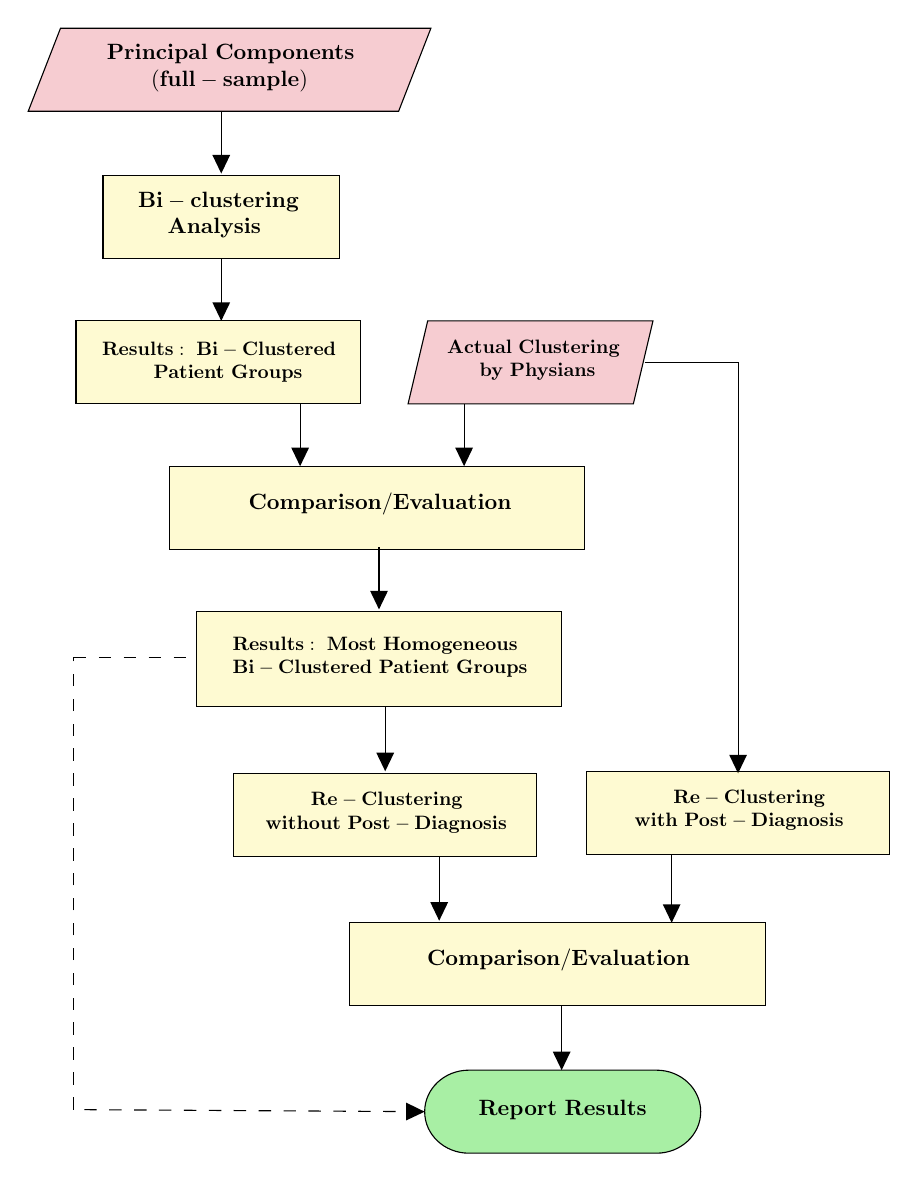
\begin{tikzpicture}[x=0.75pt,y=0.75pt,yscale=-1,xscale=1]
%uncomment if require: \path (0,606); %set diagram left start at 0, and has height of 606

%Shape: Parallelogram [id:dp6647145031150581] 
\draw  [fill={rgb, 255:red, 208; green, 2; blue, 27 }  ,fill opacity=0.2 ] (194.05,7) -- (372.5,7) -- (356.95,47) -- (178.5,47) -- cycle ;
%Straight Lines [id:da8846773602112543] 
\draw    (271.5,47) -- (271.5,75) ;
\draw [shift={(271.5,77)}, rotate = 270] [fill={rgb, 255:red, 0; green, 0; blue, 0 }  ][line width=0.75]  [draw opacity=0] (8.93,-4.29) -- (0,0) -- (8.93,4.29) -- cycle    ;

%Shape: Rectangle [id:dp27431555826277765] 
\draw  [fill={rgb, 255:red, 248; green, 231; blue, 28 }  ,fill opacity=0.2 ] (214.5,78) -- (328.5,78) -- (328.5,118) -- (214.5,118) -- cycle ;
%Straight Lines [id:da14961685906904876] 
\draw    (271.5,118) -- (271.5,146) ;
\draw [shift={(271.5,148)}, rotate = 270] [fill={rgb, 255:red, 0; green, 0; blue, 0 }  ][line width=0.75]  [draw opacity=0] (8.93,-4.29) -- (0,0) -- (8.93,4.29) -- cycle    ;

%Shape: Rectangle [id:dp09827610187608338] 
\draw  [fill={rgb, 255:red, 248; green, 231; blue, 28 }  ,fill opacity=0.2 ] (201.5,148) -- (338.5,148) -- (338.5,188) -- (201.5,188) -- cycle ;
%Straight Lines [id:da223473735957731] 
\draw    (309.5,188) -- (309.5,216) ;
\draw [shift={(309.5,218)}, rotate = 270] [fill={rgb, 255:red, 0; green, 0; blue, 0 }  ][line width=0.75]  [draw opacity=0] (8.93,-4.29) -- (0,0) -- (8.93,4.29) -- cycle    ;

%Straight Lines [id:da10156066919663931] 
\draw    (388.5,188) -- (388.5,216) ;
\draw [shift={(388.5,218)}, rotate = 270] [fill={rgb, 255:red, 0; green, 0; blue, 0 }  ][line width=0.75]  [draw opacity=0] (8.93,-4.29) -- (0,0) -- (8.93,4.29) -- cycle    ;

%Shape: Rectangle [id:dp1364397766049188] 
\draw  [fill={rgb, 255:red, 248; green, 231; blue, 28 }  ,fill opacity=0.2 ] (246.5,218) -- (446.5,218) -- (446.5,258) -- (246.5,258) -- cycle ;
%Straight Lines [id:da28849175814256767] 
\draw    (347.5,257) -- (347.5,285) ;
\draw [shift={(347.5,287)}, rotate = 270] [fill={rgb, 255:red, 0; green, 0; blue, 0 }  ][line width=0.75]  [draw opacity=0] (8.93,-4.29) -- (0,0) -- (8.93,4.29) -- cycle    ;

%Shape: Rectangle [id:dp855299838261038] 
\draw  [fill={rgb, 255:red, 248; green, 231; blue, 28 }  ,fill opacity=0.2 ] (259.5,288) -- (435.5,288) -- (435.5,334) -- (259.5,334) -- cycle ;
%Shape: Parallelogram [id:dp47004695097922267] 
\draw  [fill={rgb, 255:red, 208; green, 2; blue, 27 }  ,fill opacity=0.2 ] (370.96,148) -- (479.5,148) -- (470.04,188) -- (361.5,188) -- cycle ;
%Straight Lines [id:da06063407025060097] 
\draw    (475.5,168) -- (520.5,168) ;


%Straight Lines [id:da5926644195581223] 
\draw    (350.5,334) -- (350.5,363) ;
\draw [shift={(350.5,365)}, rotate = 270] [fill={rgb, 255:red, 0; green, 0; blue, 0 }  ][line width=0.75]  [draw opacity=0] (8.93,-4.29) -- (0,0) -- (8.93,4.29) -- cycle    ;

%Straight Lines [id:da8413098221287976] 
\draw    (520.5,168) -- (520.5,364) ;
\draw [shift={(520.5,366)}, rotate = 270] [fill={rgb, 255:red, 0; green, 0; blue, 0 }  ][line width=0.75]  [draw opacity=0] (8.93,-4.29) -- (0,0) -- (8.93,4.29) -- cycle    ;

%Shape: Rectangle [id:dp73563614757607] 
\draw  [fill={rgb, 255:red, 248; green, 231; blue, 28 }  ,fill opacity=0.2 ] (277.5,366) -- (423.5,366) -- (423.5,406) -- (277.5,406) -- cycle ;
%Shape: Rectangle [id:dp6744694293772151] 
\draw  [fill={rgb, 255:red, 248; green, 231; blue, 28 }  ,fill opacity=0.2 ] (333.5,438) -- (533.5,438) -- (533.5,478) -- (333.5,478) -- cycle ;
%Straight Lines [id:da43373610475282676] 
\draw    (376.5,406) -- (376.5,435) ;
\draw [shift={(376.5,437)}, rotate = 270] [fill={rgb, 255:red, 0; green, 0; blue, 0 }  ][line width=0.75]  [draw opacity=0] (8.93,-4.29) -- (0,0) -- (8.93,4.29) -- cycle    ;

%Straight Lines [id:da681049356627645] 
\draw    (488.5,405) -- (488.5,436) ;
\draw [shift={(488.5,438)}, rotate = 270] [fill={rgb, 255:red, 0; green, 0; blue, 0 }  ][line width=0.75]  [draw opacity=0] (8.93,-4.29) -- (0,0) -- (8.93,4.29) -- cycle    ;

%Straight Lines [id:da6627436883022095] 
\draw    (435.5,478) -- (435.5,507) ;
\draw [shift={(435.5,509)}, rotate = 270] [fill={rgb, 255:red, 0; green, 0; blue, 0 }  ][line width=0.75]  [draw opacity=0] (8.93,-4.29) -- (0,0) -- (8.93,4.29) -- cycle    ;

%Flowchart: Terminator [id:dp4539534632908053] 
\draw  [fill={rgb, 255:red, 139; green, 233; blue, 134 }  ,fill opacity=0.75 ] (390.78,509) -- (481.22,509) .. controls (492.97,509) and (502.5,517.95) .. (502.5,529) .. controls (502.5,540.05) and (492.97,549) .. (481.22,549) -- (390.78,549) .. controls (379.03,549) and (369.5,540.05) .. (369.5,529) .. controls (369.5,517.95) and (379.03,509) .. (390.78,509) -- cycle ;
%Straight Lines [id:da9928979089443342] 
\draw  [dash pattern={on 4.5pt off 4.5pt}]  (200.5,310) -- (259.5,310) ;


%Straight Lines [id:da9346137110249131] 
\draw  [dash pattern={on 4.5pt off 4.5pt}]  (200.5,528) -- (200.5,310) ;


%Straight Lines [id:da835721246834527] 
\draw  [dash pattern={on 4.5pt off 4.5pt}]  (367.5,528.99) -- (200.5,528) ;

\draw [shift={(369.5,529)}, rotate = 180.34] [fill={rgb, 255:red, 0; green, 0; blue, 0 }  ][line width=0.75]  [draw opacity=0] (8.93,-4.29) -- (0,0) -- (8.93,4.29) -- cycle    ;
%Shape: Rectangle [id:dp16102927554927304] 
\draw  [fill={rgb, 255:red, 248; green, 231; blue, 28 }  ,fill opacity=0.2 ] (447.5,365) -- (593.5,365) -- (593.5,405) -- (447.5,405) -- cycle ;

% Text Node
\draw (276,26) node [scale=0.8]  {$ \begin{array}{l}
\mathbf{Principal\ Components}\\
\ \ \ \ \ \ (\mathbf{full-sample})
\end{array}$};
% Text Node
\draw (272,97) node [scale=0.8]  {$ \begin{array}{l}
\mathbf{Bi-clustering\ }\\
\ \ \ \ \mathbf{Analysis}
\end{array}$};
% Text Node
\draw (272,168) node [scale=0.7]  {$ \begin{array}{l}
\mathbf{Results:\ Bi-Clustered\ }\\
\ \ \ \ \ \ \ \ \mathbf{Patient\ Groups}
\end{array}$};
% Text Node
\draw (422,167) node [scale=0.7]  {$ \begin{array}{l}
\mathbf{Actual\ Clustering}\\
\ \ \ \ \mathbf{\ by\ Physians}
\end{array}$};
% Text Node
\draw (348,236) node [scale=0.8]  {$\mathbf{Comparison/Evaluation}$};
% Text Node
\draw (348,310) node [scale=0.7]  {$ \begin{array}{l}
\mathbf{Results:\ Most\ Homogeneous}\\
\mathbf{Bi-Clustered\ Patient\ Groups}
\end{array}$};
% Text Node
\draw (351,385) node [scale=0.7]  {$ \begin{array}{l}
\ \ \ \ \ \ \ \mathbf{Re-Clustering\ }\\
\mathbf{without\ Post-Diagnosis}
\end{array}$};
% Text Node
\draw (434,456) node [scale=0.8]  {$\mathbf{Comparison/Evaluation}$};
% Text Node
\draw (436,528) node [scale=0.8]  {$\mathbf{Report\ Results}$};
% Text Node
\draw (521,384) node [scale=0.7]  {$ \begin{array}{l}
\ \ \ \ \ \ \mathbf{Re-Clustering\ }\\
\mathbf{with\ Post-Diagnosis}
\end{array}$};


\end{tikzpicture}

\end{minipage}
    \caption[Process flow clustering of patient groups]{\textit{Process flow clustering of patient groups}}
    \label{fig:process_flow_clustering}
\end{figure}

\subsection{The BI Clustering HF Problem}
\label{subsec:bi_clust}

In the current clustering problem we assume that the dataset is only comprised of two clusters, i.e. HFmrEF and HFpEF. Accordingly, we allow the algorithms to determine the patients that best correspond to each cluster. We have plotted the results of the BI clustering problem in Figure (\ref{fig:bi_clust_results}). This plot can in many ways seem very misguiding as it only displays the results along the two first principal components. Still, the figure illustrates that even if you only cluster based on the first four principal components (27.32\% of variance explained), one can produce more unique phenotypi-     

\begin{footnotesize}
\begin{tabularx}{1.2\textwidth}{LLLLp{1.7cm}p{3cm}}
\caption{Baseline characteristics of actual clustering}\label{tab:baseline_char_actual_full}\\
\toprule
& Total & Cluster1 & Cluster2 & $p$-value\\
\midrule
\endfirsthead
\caption*{\textbf{Table \ref{tab:baseline_char_actual_full}:} Baseline characteristics of actual clustering (\textit{continued})}\\
\toprule
& Total & Cluster1 & Cluster2 & $p$-value\\
\midrule
\endhead
hb & 109.34±20.29 & 107.85±21.22 & 110.93±19.18 & 0.141 \\ 
pcv & 0.34±0.06 & 0.33±0.06 & 0.34±0.06 & 0.159 \\ 
age & 78.64(69.22,84.17) & 78.9(69.46,85.37) & 78.08(68.73,82.74) & 0.141 \\ 
ewave & 0.9(0.74,1.05) & 0.92(0.8,1.1) & 0.9(0.7,1.01) & 0.056 \\ 
gfr & 48(32.5,70) & 47(32,72) & 51.96(33,67.77) & 0.968 \\ 
k & 4.4(4,4.7) & 4.4(4.1,4.7) & 4.4(4,4.78) & 0.664 \\ 
los & 10(4,22) & 10(4,22) & 10.5(4,21) & 0.880 \\ 
lvef & 50(45,57.5) & 57.5(55,60) & 45(42,47.5) & 0.000*** \\ 
mcv & 90.55(85.5,95) & 89(85,94) & 91.33(87,96) & 0.011** \\ 
na & 139(136,141) & 139(136,141) & 139(136,141) & 0.650 \\ 
ntprobnp & 2848(1230.5,7374) & 2217(997,5305) & 4063.5(1886.5,9968.25) & 0.000*** \\ 
plts & 204(156,268) & 217(163,284) & 190.87(148.5,241) & 0.003** \\ 
wbc & 7.8(5.9,10.5) & 7.6(6,10.5) & 8.1(5.9,10.4) & 0.727 \\ 
\midrule
\multicolumn{3}{l}{Total number of significant baseline char:} & 59\\
\multicolumn{3}{l}{\hspace*{0,5cm} Continuous: } & 4\\
\multicolumn{3}{l}{\hspace*{0,5cm} Categorical: } & 55\\
\midrule
\end{tabularx}
\end{footnotesize}

\begin{footnotesize}
\begin{tabularx}{1.2\textwidth}{LLLLp{1.7cm}p{3cm}}
\caption{Baseline characteristics of Hierarchical and K-Means clustering}\label{tab:baseline_char_actual_hckm}\\
\toprule
& Total & Cluster1 & Cluster2 & $p$-value\\
\midrule
\endfirsthead
\caption*{\textbf{Table \ref{tab:baseline_char_actual_hckm}:} Baseline characteristics of Hierarchical and K-Means clustering (\textit{continued})}\\
\toprule
& Total & Cluster1 & Cluster2 & $p$-value\\
\midrule
\endhead
hb & 109.34±20.29 & 106.79±21.29 & 111.73±19.06 & 0.019** \\ 
pcv & 0.34±0.06 & 0.33±0.07 & 0.35±0.06 & 0.035* \\ 
age & 78.64(69.22,84.17) & 78.9(68.94,85.36) & 78.26(69.73,82.8) & 0.416 \\ 
ewave & 0.9(0.74,1.05) & 0.97(0.8,1.1) & 0.9(0.7,1) & 0.002** \\ 
gfr & 48(32.5,70) & 46(31,70) & 54.44(34,71) & 0.205 \\ 
k & 4.4(4,4.7) & 4.4(4,4.7) & 4.4(4,4.8) & 0.219 \\ 
los & 10(4,22) & 10(4,22) & 11(4.25,21) & 0.889 \\ 
lvef & 50(45,57.5) & 57.5(52.5,60) & 45(42.5,47.5) & 0.000*** \\ 
mcv & 90.55(85.5,95) & 89(84,94) & 91.14(87,96) & 0.002** \\ 
na & 139(136,141) & 139(136,141) & 139(136,141) & 0.321 \\ 
ntprobnp & 2848(1230.5,7374) & 2327(1007,5695) & 3723.5(1731.5,9557.75) & 0.000*** \\ 
plts & 204(156,268) & 215(163,287) & 194(151,241) & 0.007** \\ 
wbc & 7.8(5.9,10.5) & 7.7(5.9,10.5) & 8.05(5.92,10.47) & 0.731 \\ 
\midrule
\multicolumn{3}{l}{Total number of significant baseline char:} & 62\\
\multicolumn{3}{l}{\hspace*{0,5cm} Continuous: } & 7\\
\multicolumn{3}{l}{\hspace*{0,5cm} Categorical: } & 55\\
\midrule
\end{tabularx}
\end{footnotesize}

\noindent cally distinct patient groups than the physicians. As we can see from table (\ref{tab:baseline_char_actual_hckm}), the  Hierarchical and K-Means clustering algorithms both give the highest number of significant baseline characteristics (7 for only the cont. variables in the table and 62 in total) compared with the actual clustering done by the physicians (4 for the cont. variables and 59 in total, see table \ref{tab:baseline_char_actual_full}). The EM algorithm produces overall the lowest number of significant baseline characteristics (5 for cont. variables and 54 in total). Both the Hierarchical and K-Means algorithm produce the same clustering configurations. The baseline characteristics in the clustering of the patient using the Hierarchical and K-Means clustering show that for the first clustering (HFpEF) the \texttt{LVEF} is on average 57.5\% and for the second clustering (HFmrEF) the \texttt{LVEF} is on average 45\%. These are very similar values as that which was done by the physicians. We can also see for other baseline characteristics such as \texttt{ntprobnp} the average is at 2327 ng/L for the HFpEF group which is significantly different than that of the HFmrEF group 3723.5 ng/L, also this is very similar to what the physicians concluded with. For characteristics that are significantly different in the clustering with Hierarchical and K-Means, but not found in the clustering done by the physicians one can include the following continuous variables: hemoglobin (\texttt{hb}), packed cell volume (\texttt{pcv}) and the ewave (\texttt{ewave}). This may suggest that both the cluste-    

\begin{footnotesize}
\begin{tabularx}{1.2\textwidth}{LLLLp{1.7cm}p{3cm}}
\caption{Baseline characteristics of EM clustering}\label{tab:baseline_char_actual_em}\\
\toprule
& Total & Cluster1 & Cluster2 & $p$-value\\
\midrule
\endfirsthead
\caption*{\textbf{Table \ref{tab:baseline_char_actual_em}:} Baseline characteristics of EM clustering (\textit{continued})}\\
\toprule
& Total & Cluster1 & Cluster2 & $p$-value\\
\midrule
\endhead
hb & 109.34±20.29 & 111.2±19.07 & 107.48±21.34 & 0.075 \\ 
pcv & 0.34±0.06 & 0.34±0.06 & 0.33±0.06 & 0.115 \\ 
age & 78.64(69.22,84.17) & 77.81(69.22,82.76) & 78.9(69.22,85.36) & 0.199 \\ 
ewave & 0.9(0.74,1.05) & 0.9(0.71,1.01) & 0.93(0.8,1.1) & 0.040* \\ 
gfr & 48(32.5,70) & 51.96(33,68.25) & 47(32,72) & 0.956 \\ 
k & 4.4(4,4.7) & 4.4(4,4.8) & 4.4(4,4.7) & 0.363 \\ 
los & 10(4,22) & 11(4,21) & 10(4,22) & 0.906 \\ 
lvef & 50(45,57.5) & 45(42,47.5) & 57.5(53.75,60) & 0.000*** \\ 
mcv & 90.55(85.5,95) & 91.14(87,96) & 89(84.5,94) & 0.007** \\ 
na & 139(136,141) & 139(136,141) & 139(136,141) & 0.330 \\ 
ntprobnp & 2848(1230.5,7374) & 3985(1849.5,10038.25) & 2226(990,5500) & 0.000*** \\ 
plts & 204(156,268) & 192.64(149.5,241.5) & 217(163.5,286) & 0.002** \\ 
wbc & 7.8(5.9,10.5) & 8.1(5.97,10.63) & 7.6(5.9,10.35) & 0.561 \\ 
\midrule
\multicolumn{3}{l}{Total number of significant baseline char:} & 54\\
\multicolumn{3}{l}{\hspace*{0,5cm} Continuous: } & 5\\
\multicolumn{3}{l}{\hspace*{0,5cm} Categorical: } & 49\\
\midrule
\end{tabularx}
\end{footnotesize}

\noindent ring algorithms, i.e. HC and KM can be used as appropriate tools for physicians. The results from the EM algorithm (Table \ref{tab:baseline_char_actual_em}) show that a lot of the similar baseline characteristics are not statistically significant. The LVEF (\texttt{lvef}) and NTproBNP (\texttt{ntprobnp}) is very similar to both the Hierarchical and K-means clustering, but other characteristics such as hemoglobin (\texttt{hb}) and the packed cell volume (\texttt{pcv}) are not. Throughout the analysis we have found that the EM algorithm does not a good job of clustering patient groups compared to the Hierarchical and K-Means clustering algorithms. This could be because of the assumption of multivariate normal distribution does not hold for this data set or the fact that there is a high presence of categorical variables in the data set.

\subsection{Analysis of Post-Diagnosis}

\noindent In this section we will investigate the clustering results discussed previously. We have place an assumption of whether the physicians diagnosis is representative given an objective of producing the most unique patient groups. The clustering problem in this section assumes that the diagnosis done by the physicians is sufficient in regards to this objective, i.e. the clustering based on the \textit{post-diagnosis} done by the physicians produces the  

\begin{footnotesize}
\begin{tabularx}{1.2\textwidth}{Lcccc}
\caption{Number of significant baseline characteristics}\label{tab:n_baseline}\\
\toprule
& \multicolumn{2}{c}{With Post-Diagnosis} & \multicolumn{2}{c}{Without Post-Diagnosis}\\
& HFpEF & HFmrEF & HFpEF & HFmrEF\\
\midrule
\endfirsthead
\caption*{\textbf{Table \ref{tab:n_baseline}:} Number of significant baseline characteristics (\textit{continued})}\\
\toprule
& \multicolumn{2}{c}{With Post-Diagnosis} & \multicolumn{2}{c}{Without Post-Diagnosis}\\
& HFpEF & HFmrEF & HFpEF & HFmrEF\\
\midrule
\endhead
Hierarchical &  53 (tab. \ref{tab:baseline_char_phy_p_hc}) &  53 (tab. \ref{tab:baseline_char_phy_mr_hc}) &  48 (tab. \ref{tab:baseline_char_nophy_p_hc}) &  51 (tab. \ref{tab:baseline_char_nophy_mr_hc})\\ 
K-Means &  49 (tab. \ref{tab:baseline_char_phy_p_km}) &  53 (tab. \ref{tab:baseline_char_phy_mr_km}) &  48 (tab. \ref{tab:baseline_char_nophy_p_km}) &  53 (tab. \ref{tab:baseline_char_nophy_mr_km})\\ 
EM &  56 (tab. \ref{tab:baseline_char_phy_p_em}) &  44 (tab. \ref{tab:baseline_char_phy_mr_em}) &  42 (tab. \ref{tab:baseline_char_nophy_p_em}) &  42 (tab. \ref{tab:baseline_char_nophy_mr_em})\\ 
\midrule
\end{tabularx}
\end{footnotesize}

\noindent most unique patient groups. We compare these results to a clustering without an assumption of post-diagnosis done by the physicians and see if there are any substantial differences in results. We will only use the first two principal components (14.64\% of variance explained) to cluster the patients. The evaluation criteria is the same as in the previous section. Accordingly, we can see from Table (\ref{tab:n_baseline}) that the Hierarchical and K-Means clustering algorithms produces the same number of significant baseline characteristics in half of the cases examined.  We can also see from Table (\ref{tab:n_baseline}) that all algorithms analyzed produce on average more statistically significant baseline characteristics with the post-diagnosis assumption compared to without. The EM algorithm produces overall the lowest number of significant baseline characteristics (in three cases). An exception is when the EM algorithm is clustering HFpEF with post-diagnosis.\\ 
\indent Starting out with the subtype HFpEF given the assumption of post-diagnosis, we can see from tables (\ref{tab:baseline_char_phy_p_hc}) and (\ref{tab:baseline_char_phy_p_km}) that cluster 2 (Hierarchical \& K-Means) seems to contain patients that have a higher average \texttt{age} (85.45) with a packed cell volume (\texttt{pcv}) that is on average 0.33 $\pm$ 0.05. This cluster is very similar to cluster 1 produced by the EM algorithm. The ntprobnp (\texttt{ntprobnp}) of cluster 3 (Hierarchical \& K-Means) is the lowest at 1417 ng/L which is also statistically significant. The average number of red blood cells, i.e. the mean corpusular volume (\texttt{mcv}) is at its lowest for cluster 1 (Hierarchical \& K-means) with an average of 87 femtolitres. The number of significant baseline characteristics produced by the Hierarchical clustering is 53 (8 cont. and 48 categorical) and for the K-Means its 49 (8 cont. and 41 categorical). The EM algorithm produces almost similar results for the subgroup HFpEF as the Hierarchical and K-Means algorithm (table \ref{tab:baseline_char_phy_p_em}). The second cluster produced by the EM algorithm is very similar to the third cluster produced by the Hierarchical and the K-Means algorithm. The ntprobnp (\texttt{ntprobnp}) for cluster one and two produced by the EM are very similar. Both are approximately 2750 ng/L. The third cluster produced by the EM algorithm has the lowest values for the ntprobnp (1525 nl/L). The total number of significant baseline characteristics for the EM algorithm is 56 (8 cont. and 48 categorical). \\ 
\indent When looking at the HFmrEF clustering based on post-diagnosis (tables \ref{tab:baseline_char_phy_mr_hc}, \ref{tab:baseline_char_phy_mr_km} and \ref{tab:baseline_char_phy_mr_em}), we can see that a somewhat different results shows up, i.e. there are on average less significantly different baseline characteristics in all clusters produced by the algorithms regardless of whether the assumption of post-diagnosis is intact. For cluster 3 (Hierarchical and K-Means), we find the lowest ntprobnp (\texttt{ntprobnp}) at 2898.5 ng/L with a packed cell volume of 0.38 $\pm$ 0.04. This cluster also contains the patients with the lowest length of stay (7 days). The length of stay (\texttt{LOS}) is also a uniquely statistical significant baseline characteristic that is only significant in the HFmrEF subgroup of patients for all algorithms studied. Cluster 3 also has the highest hemoglobin (\texttt{hb}) at 123.79 $\pm$ 12.89 g/100mL. The clustering results without the post-diagnosis assumption shows very different results. In general, Figure (\ref{fig:clust_results_without_post_p}) and (\ref{fig:clust_results_without_post_mr}) show that the assignment of clustering happens with very little similarities, i.e. the cluster numbering as well as the baseline characteristics vary more when the assumption of post-diagnosis is removed. Comparing the number of significant baseline characteristics between the HFmrEF groups both with and without the post-diagnosis assumption shows that the latter has on average fewer baseline characteristics, see table (\ref{tab:n_baseline}). The same goes for the HFpEF group, i.e. we have reasons to believe that assuming the physicians diagnosis is representative, one can get additional clustered patient groups with higher degree of homogeneity compared to when this assumption is not intact. We have also demonstrated that the ML algorithms can be very useful in producing patient groups that are more phenotypically unique given that the objective is to challenge the diagnosis of the physicians, see section (\ref{subsec:bi_clust}). Now that we have presented the results of the clustering analysis, we move on to the results of the classification of the clinical outcomes. The source code, relevant plots and tables can be found in the appendix (\ref{chap:data_desc}).

\vspace*{-0,5cm}\section{Classification}

\noindent In this section we will present the results of the classification analysis. As mentioned in ML the procedure (figure \ref{fig:ML_proc_thesis}), we run the imputed data set through the various classification algorithms and accordingly run a cross validation in order to estimate the accuracy of the various algorithms. The accuracy along with Cohen’s kappa are the two evaluation criteria we use to rank the algorithms in this section. The process flow for the mentioned classification section is illustrated in Figure (\ref{fig:process_flow_classification}). 

\begin{figure}
    \centering
    \begin{minipage}[b]{\textwidth}

\centering
\normalsize

\tikzset{every picture/.style={line width=0.75pt}} %set default line width to 0.75pt        

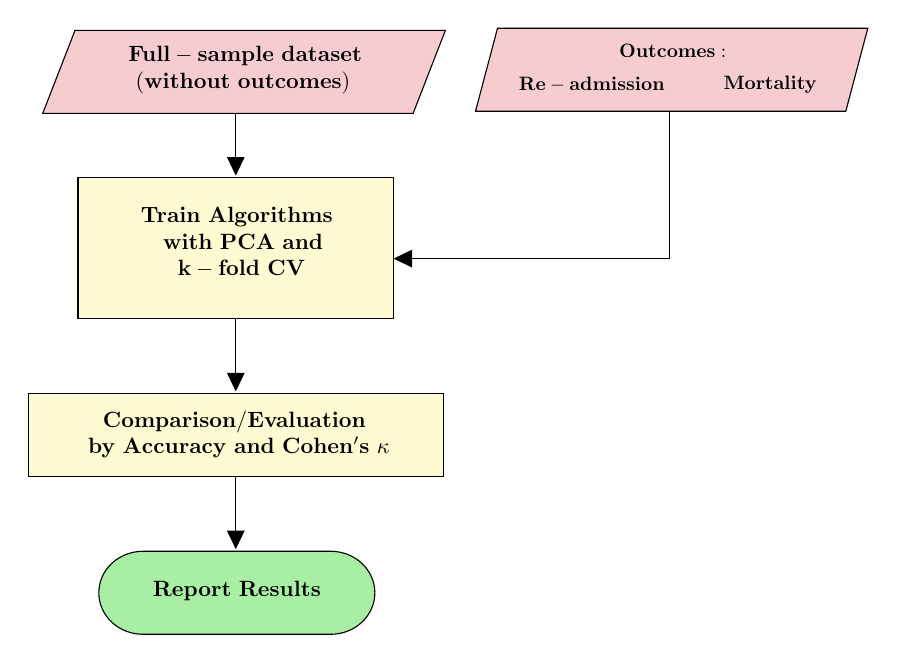
\begin{tikzpicture}[x=0.75pt,y=0.75pt,yscale=-1,xscale=1]
%uncomment if require: \path (0,401); %set diagram left start at 0, and has height of 401

%Shape: Parallelogram [id:dp1345085496641345] 
\draw  [fill={rgb, 255:red, 208; green, 2; blue, 27 }  ,fill opacity=0.2 ] (214.05,27) -- (392.5,27) -- (376.95,67) -- (198.5,67) -- cycle ;
%Straight Lines [id:da2529734460759472] 
\draw    (291.5,67) -- (291.5,95) ;
\draw [shift={(291.5,97)}, rotate = 270] [fill={rgb, 255:red, 0; green, 0; blue, 0 }  ][line width=0.75]  [draw opacity=0] (8.93,-4.29) -- (0,0) -- (8.93,4.29) -- cycle    ;

%Shape: Rectangle [id:dp8537246297754715] 
\draw  [fill={rgb, 255:red, 248; green, 231; blue, 28 }  ,fill opacity=0.2 ] (215.5,98) -- (367.5,98) -- (367.5,166) -- (215.5,166) -- cycle ;
%Shape: Parallelogram [id:dp3026993474655866] 
\draw  [fill={rgb, 255:red, 208; green, 2; blue, 27 }  ,fill opacity=0.2 ] (417.6,26) -- (596,26) -- (585.4,66) -- (407,66) -- cycle ;
%Straight Lines [id:da11621318058538299] 
\draw    (500.5,66) -- (500.5,137) ;


%Straight Lines [id:da5046262970656357] 
\draw    (369.5,137) -- (500.5,137) ;

\draw [shift={(367.5,137)}, rotate = 0] [fill={rgb, 255:red, 0; green, 0; blue, 0 }  ][line width=0.75]  [draw opacity=0] (8.93,-4.29) -- (0,0) -- (8.93,4.29) -- cycle    ;
%Shape: Rectangle [id:dp6205627904748299] 
\draw  [fill={rgb, 255:red, 248; green, 231; blue, 28 }  ,fill opacity=0.2 ] (191.5,202) -- (391.5,202) -- (391.5,242) -- (191.5,242) -- cycle ;
%Straight Lines [id:da7285903815225594] 
\draw    (291.5,166) -- (291.5,199) ;
\draw [shift={(291.5,201)}, rotate = 270] [fill={rgb, 255:red, 0; green, 0; blue, 0 }  ][line width=0.75]  [draw opacity=0] (8.93,-4.29) -- (0,0) -- (8.93,4.29) -- cycle    ;

%Straight Lines [id:da5366229358958934] 
\draw    (291.5,242) -- (291.5,275) ;
\draw [shift={(291.5,277)}, rotate = 270] [fill={rgb, 255:red, 0; green, 0; blue, 0 }  ][line width=0.75]  [draw opacity=0] (8.93,-4.29) -- (0,0) -- (8.93,4.29) -- cycle    ;

%Flowchart: Terminator [id:dp45661416532888843] 
\draw  [fill={rgb, 255:red, 139; green, 233; blue, 134 }  ,fill opacity=0.75 ] (246.78,278) -- (337.22,278) .. controls (348.97,278) and (358.5,286.95) .. (358.5,298) .. controls (358.5,309.05) and (348.97,318) .. (337.22,318) -- (246.78,318) .. controls (235.03,318) and (225.5,309.05) .. (225.5,298) .. controls (225.5,286.95) and (235.03,278) .. (246.78,278) -- cycle ;

% Text Node
\draw (296,46) node [scale=0.8]  {$ \begin{array}{l}
\mathbf{Full-sample\ dataset}\\
\mathbf{\ ( without\ outcomes)}
\end{array}$};
% Text Node
\draw (292,130) node [scale=0.8]  {$ \begin{array}{l}
\mathbf{Train\ Algorithms}\\
\ \ \ \mathbf{with\ PCA\ and\ }\\
\ \ \ \ \ \mathbf{k-fold\ CV}
\end{array}$};
% Text Node
\draw (463,53) node [scale=0.7]  {$\mathbf{Re-admission}$};
% Text Node
\draw (549,53) node [scale=0.7]  {$\mathbf{Mortality}$};
% Text Node
\draw (502,37) node [scale=0.7]  {$\mathbf{Outcomes:}$};
% Text Node
\draw (293,222) node [scale=0.8]  {$ \begin{array}{l}
\ \ \mathbf{Comparison/Evaluation}\\
\mathbf{by\ Accuracy\ and\ Cohen's\ \kappa }
\end{array}$};
% Text Node
\draw (292,297) node [scale=0.8]  {$\mathbf{Report\ Results}$};

\end{tikzpicture}


\end{minipage}
    \caption[Process flow classification of clinical outcomes]{\textit{Process flow classification of clinical outcomes}}
    \label{fig:process_flow_classification}
\end{figure}

\subsection{Mortality Classifier}

\noindent The statistical learning problem in this section is given by a two-class classification problem where mortality is the clinical outcome in question. Our objective is to see how well the algorithms mentioned in Figure (\ref{fig:ML_proc_thesis}) perform in predicting the probability of mortality. We will train the algorithms using $5$-fold cross validation and evaluate the results using the accuracy, i.e. the proportion of true results and the Cohen's kappa defined by:
\begin{align}
    \kappa \equiv \frac{p_0 - p_e}{1 - p_e}
\end{align}
where $p_0$ is the accuracy given by ${\mathit  {ACC}}=({\mathit  {TP}}+{\mathit  {TN}})/(P+N)$, and $p_e = 1 / N^2 \sum_{k} n_{k1}n_{k2}$, where $k$ is the number of categories / classes, $N$ the number of items and $n_{k1}$ the number of times rater $i$ predicted category $k$. $p_e$ is also referred to as the expected accuracy, i.e. what the accuracy that any \textit{random} classifier would be expected to achieve. Accordingly, Cohen's kappa is also regarded as the inter-rater agreement for qualitative (categorical) items, i.e. it is like classification accuracy, except that it is normalized at the baseline of random chance on a dataset. A possible interpretation of this statistics is given in by the following \citep{ashby1991practical}: less than 0.20 = Poor agreement, 0.20 to 0.40 = Fair agreement, 0.40 to 0.60 = Moderate agreement, 0.60 to 0.80 = Good agreement and 0.80 to 1 = Very good agreement. As mentioned earlier, the statistical learning problem is that of a Binary classification problem given by whether  re-admission / mortality occurred (\texttt{TRUE}) or not (\texttt{FALSE}), i.e. the expected accuracy is $p_e = 0.50$. The total number of patients with post-confirmed mortality in this data set is 115 (approx 36\% of the total number of patients, see table \ref{tab:outcomes_class}). In addition to the classifica-

\begin{figure}[h!]
    \centering
    \scalebox{.8}{% Created by tikzDevice version 0.11 on 2018-10-22 23:22:36
% !TEX encoding = UTF-8 Unicode
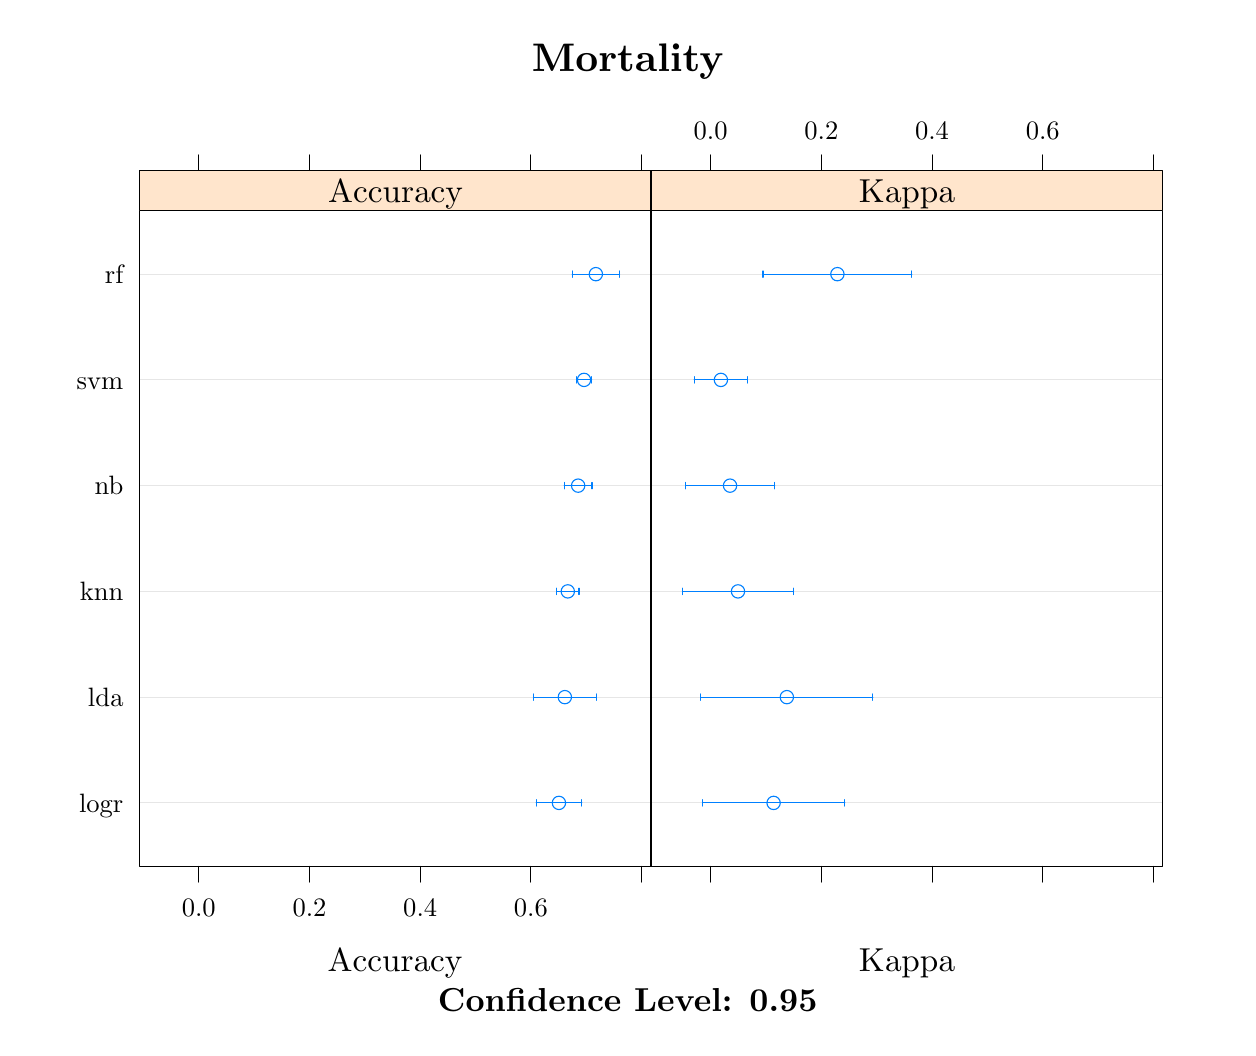
\begin{tikzpicture}[x=1pt,y=1pt]
\definecolor{fillColor}{RGB}{255,255,255}
\path[use as bounding box,fill=fillColor,fill opacity=0.00] (0,0) rectangle (433.62,361.35);
\begin{scope}
\path[clip] (  0.00,  0.00) rectangle (433.62,361.35);

\path[] (  0.00,  0.00) rectangle (433.62,361.35);
\definecolor{drawColor}{RGB}{0,0,0}

\node[text=drawColor,anchor=base,inner sep=0pt, outer sep=0pt, scale=  1.44] at (216.81,345.39) {\bfseries Mortality};
\end{scope}
\begin{scope}
\path[clip] (  0.00,  0.00) rectangle (433.62,361.35);
\definecolor{drawColor}{RGB}{0,0,0}

\node[text=drawColor,anchor=base,inner sep=0pt, outer sep=0pt, scale=  1.20] at (216.81,  6.02) {\bfseries Confidence Level: 0.95};
\end{scope}
\begin{scope}
\path[clip] (  0.00,  0.00) rectangle (433.62,361.35);
\definecolor{drawColor}{RGB}{0,0,0}

\node[text=drawColor,anchor=base,inner sep=0pt, outer sep=0pt, scale=  1.20] at (132.76, 20.33) {Accuracy};

\node[text=drawColor,anchor=base,inner sep=0pt, outer sep=0pt, scale=  1.20] at (317.71, 20.33) {Kappa};
\end{scope}
\begin{scope}
\path[clip] (  0.00,  0.00) rectangle (433.62,361.35);
\definecolor{drawColor}{RGB}{0,0,0}

\path[draw=drawColor,line width= 0.4pt,line join=round,line cap=round] ( 61.84,309.66) -- ( 61.84,315.35);

\path[draw=drawColor,line width= 0.4pt,line join=round,line cap=round] (101.84,309.66) -- (101.84,315.35);

\path[draw=drawColor,line width= 0.4pt,line join=round,line cap=round] (141.84,309.66) -- (141.84,315.35);

\path[draw=drawColor,line width= 0.4pt,line join=round,line cap=round] (181.84,309.66) -- (181.84,315.35);

\path[draw=drawColor,line width= 0.4pt,line join=round,line cap=round] (221.84,309.66) -- (221.84,315.35);
\end{scope}
\begin{scope}
\path[clip] (  0.00,  0.00) rectangle (433.62,361.35);
\definecolor{drawColor}{RGB}{0,0,0}

\node[text=drawColor,anchor=base east,inner sep=0pt, outer sep=0pt, scale=  0.96] at ( 34.58, 77.92) {logr};

\node[text=drawColor,anchor=base east,inner sep=0pt, outer sep=0pt, scale=  0.96] at ( 34.58,116.13) {lda};

\node[text=drawColor,anchor=base east,inner sep=0pt, outer sep=0pt, scale=  0.96] at ( 34.58,154.34) {knn};

\node[text=drawColor,anchor=base east,inner sep=0pt, outer sep=0pt, scale=  0.96] at ( 34.58,192.55) {nb};

\node[text=drawColor,anchor=base east,inner sep=0pt, outer sep=0pt, scale=  0.96] at ( 34.58,230.76) {svm};

\node[text=drawColor,anchor=base east,inner sep=0pt, outer sep=0pt, scale=  0.96] at ( 34.58,268.97) {rf};
\end{scope}
\begin{scope}
\path[clip] (  0.00,  0.00) rectangle (433.62,361.35);
\definecolor{drawColor}{RGB}{0,0,0}

\path[draw=drawColor,line width= 0.4pt,line join=round,line cap=round] ( 61.84, 58.30) -- ( 61.84, 52.61);

\path[draw=drawColor,line width= 0.4pt,line join=round,line cap=round] (101.84, 58.30) -- (101.84, 52.61);

\path[draw=drawColor,line width= 0.4pt,line join=round,line cap=round] (141.84, 58.30) -- (141.84, 52.61);

\path[draw=drawColor,line width= 0.4pt,line join=round,line cap=round] (181.84, 58.30) -- (181.84, 52.61);

\path[draw=drawColor,line width= 0.4pt,line join=round,line cap=round] (221.84, 58.30) -- (221.84, 52.61);

\node[text=drawColor,anchor=base,inner sep=0pt, outer sep=0pt, scale=  0.96] at ( 61.84, 40.30) {0.0};

\node[text=drawColor,anchor=base,inner sep=0pt, outer sep=0pt, scale=  0.96] at (101.84, 40.30) {0.2};

\node[text=drawColor,anchor=base,inner sep=0pt, outer sep=0pt, scale=  0.96] at (141.84, 40.30) {0.4};

\node[text=drawColor,anchor=base,inner sep=0pt, outer sep=0pt, scale=  0.96] at (181.84, 40.30) {0.6};
\end{scope}
\begin{scope}
\path[clip] ( 40.28, 58.30) rectangle (225.23,295.21);
\definecolor{drawColor}{RGB}{230,230,230}

\path[draw=drawColor,line width= 0.4pt,line join=round,line cap=round] ( 40.28, 81.22) -- (225.23, 81.22);

\path[draw=drawColor,line width= 0.4pt,line join=round,line cap=round] ( 40.28,119.44) -- (225.23,119.44);

\path[draw=drawColor,line width= 0.4pt,line join=round,line cap=round] ( 40.28,157.65) -- (225.23,157.65);

\path[draw=drawColor,line width= 0.4pt,line join=round,line cap=round] ( 40.28,195.86) -- (225.23,195.86);

\path[draw=drawColor,line width= 0.4pt,line join=round,line cap=round] ( 40.28,234.07) -- (225.23,234.07);

\path[draw=drawColor,line width= 0.4pt,line join=round,line cap=round] ( 40.28,272.28) -- (225.23,272.28);
\definecolor{drawColor}{RGB}{0,128,255}

\path[draw=drawColor,line width= 0.4pt,line join=round,line cap=round] (191.97, 81.22) circle (  2.41);

\path[draw=drawColor,line width= 0.4pt,line join=round,line cap=round] (194.11,119.44) circle (  2.41);

\path[draw=drawColor,line width= 0.4pt,line join=round,line cap=round] (195.17,157.65) circle (  2.41);

\path[draw=drawColor,line width= 0.4pt,line join=round,line cap=round] (198.91,195.86) circle (  2.41);

\path[draw=drawColor,line width= 0.4pt,line join=round,line cap=round] (201.04,234.07) circle (  2.41);

\path[draw=drawColor,line width= 0.4pt,line join=round,line cap=round] (205.31,272.28) circle (  2.41);

\path[draw=drawColor,line width= 0.4pt,line join=round,line cap=round] (183.73, 81.22) -- (200.22, 81.22);

\path[draw=drawColor,line width= 0.4pt,line join=round,line cap=round] (182.73,119.44) -- (205.48,119.44);

\path[draw=drawColor,line width= 0.4pt,line join=round,line cap=round] (191.12,157.65) -- (199.23,157.65);

\path[draw=drawColor,line width= 0.4pt,line join=round,line cap=round] (193.89,195.86) -- (203.93,195.86);

\path[draw=drawColor,line width= 0.4pt,line join=round,line cap=round] (198.27,234.07) -- (203.81,234.07);

\path[draw=drawColor,line width= 0.4pt,line join=round,line cap=round] (196.74,272.28) -- (213.88,272.28);

\path[draw=drawColor,line width= 0.4pt,line join=round,line cap=round] (183.73, 82.37) -- (183.73, 80.08);

\path[draw=drawColor,line width= 0.4pt,line join=round,line cap=round] (182.73,120.58) -- (182.73,118.29);

\path[draw=drawColor,line width= 0.4pt,line join=round,line cap=round] (191.12,158.79) -- (191.12,156.50);

\path[draw=drawColor,line width= 0.4pt,line join=round,line cap=round] (193.89,197.00) -- (193.89,194.71);

\path[draw=drawColor,line width= 0.4pt,line join=round,line cap=round] (198.27,235.22) -- (198.27,232.92);

\path[draw=drawColor,line width= 0.4pt,line join=round,line cap=round] (196.74,273.43) -- (196.74,271.13);

\path[draw=drawColor,line width= 0.4pt,line join=round,line cap=round] (200.22, 82.37) -- (200.22, 80.08);

\path[draw=drawColor,line width= 0.4pt,line join=round,line cap=round] (205.48,120.58) -- (205.48,118.29);

\path[draw=drawColor,line width= 0.4pt,line join=round,line cap=round] (199.23,158.79) -- (199.23,156.50);

\path[draw=drawColor,line width= 0.4pt,line join=round,line cap=round] (203.93,197.00) -- (203.93,194.71);

\path[draw=drawColor,line width= 0.4pt,line join=round,line cap=round] (203.81,235.22) -- (203.81,232.92);

\path[draw=drawColor,line width= 0.4pt,line join=round,line cap=round] (213.88,273.43) -- (213.88,271.13);
\end{scope}
\begin{scope}
\path[clip] (  0.00,  0.00) rectangle (433.62,361.35);
\definecolor{drawColor}{RGB}{0,0,0}

\path[draw=drawColor,line width= 0.4pt,line join=round,line cap=round] ( 40.28, 58.30) rectangle (225.23,295.21);
\end{scope}
\begin{scope}
\path[clip] ( 40.28,295.21) rectangle (225.23,309.66);
\definecolor{drawColor}{RGB}{255,229,204}
\definecolor{fillColor}{RGB}{255,229,204}

\path[draw=drawColor,line width= 0.4pt,line join=round,line cap=round,fill=fillColor] ( 40.28,295.21) rectangle (225.23,309.66);
\definecolor{drawColor}{RGB}{0,0,0}

\node[text=drawColor,anchor=base west,inner sep=0pt, outer sep=0pt, scale=  1.20] at (108.58,298.30) {Accuracy};
\end{scope}
\begin{scope}
\path[clip] (  0.00,  0.00) rectangle (433.62,361.35);
\definecolor{drawColor}{RGB}{0,0,0}

\path[draw=drawColor,line width= 0.4pt,line join=round,line cap=round] ( 40.28,295.21) rectangle (225.23,309.66);
\end{scope}
\begin{scope}
\path[clip] (  0.00,  0.00) rectangle (433.62,361.35);
\definecolor{drawColor}{RGB}{0,0,0}

\path[draw=drawColor,line width= 0.4pt,line join=round,line cap=round] (246.80,309.66) -- (246.80,315.35);

\path[draw=drawColor,line width= 0.4pt,line join=round,line cap=round] (286.80,309.66) -- (286.80,315.35);

\path[draw=drawColor,line width= 0.4pt,line join=round,line cap=round] (326.80,309.66) -- (326.80,315.35);

\path[draw=drawColor,line width= 0.4pt,line join=round,line cap=round] (366.80,309.66) -- (366.80,315.35);

\path[draw=drawColor,line width= 0.4pt,line join=round,line cap=round] (406.80,309.66) -- (406.80,315.35);

\node[text=drawColor,anchor=base,inner sep=0pt, outer sep=0pt, scale=  0.96] at (246.80,321.04) {0.0};

\node[text=drawColor,anchor=base,inner sep=0pt, outer sep=0pt, scale=  0.96] at (286.80,321.04) {0.2};

\node[text=drawColor,anchor=base,inner sep=0pt, outer sep=0pt, scale=  0.96] at (326.80,321.04) {0.4};

\node[text=drawColor,anchor=base,inner sep=0pt, outer sep=0pt, scale=  0.96] at (366.80,321.04) {0.6};
\end{scope}
\begin{scope}
\path[clip] (  0.00,  0.00) rectangle (433.62,361.35);
\definecolor{drawColor}{RGB}{0,0,0}

\path[draw=drawColor,line width= 0.4pt,line join=round,line cap=round] (246.80, 58.30) -- (246.80, 52.61);

\path[draw=drawColor,line width= 0.4pt,line join=round,line cap=round] (286.80, 58.30) -- (286.80, 52.61);

\path[draw=drawColor,line width= 0.4pt,line join=round,line cap=round] (326.80, 58.30) -- (326.80, 52.61);

\path[draw=drawColor,line width= 0.4pt,line join=round,line cap=round] (366.80, 58.30) -- (366.80, 52.61);

\path[draw=drawColor,line width= 0.4pt,line join=round,line cap=round] (406.80, 58.30) -- (406.80, 52.61);
\end{scope}
\begin{scope}
\path[clip] (225.23, 58.30) rectangle (410.19,295.21);
\definecolor{drawColor}{RGB}{230,230,230}

\path[draw=drawColor,line width= 0.4pt,line join=round,line cap=round] (225.23, 81.22) -- (410.19, 81.22);

\path[draw=drawColor,line width= 0.4pt,line join=round,line cap=round] (225.23,119.44) -- (410.19,119.44);

\path[draw=drawColor,line width= 0.4pt,line join=round,line cap=round] (225.23,157.65) -- (410.19,157.65);

\path[draw=drawColor,line width= 0.4pt,line join=round,line cap=round] (225.23,195.86) -- (410.19,195.86);

\path[draw=drawColor,line width= 0.4pt,line join=round,line cap=round] (225.23,234.07) -- (410.19,234.07);

\path[draw=drawColor,line width= 0.4pt,line join=round,line cap=round] (225.23,272.28) -- (410.19,272.28);
\definecolor{drawColor}{RGB}{0,128,255}

\path[draw=drawColor,line width= 0.4pt,line join=round,line cap=round] (269.54, 81.22) circle (  2.41);

\path[draw=drawColor,line width= 0.4pt,line join=round,line cap=round] (274.33,119.44) circle (  2.41);

\path[draw=drawColor,line width= 0.4pt,line join=round,line cap=round] (256.67,157.65) circle (  2.41);

\path[draw=drawColor,line width= 0.4pt,line join=round,line cap=round] (253.80,195.86) circle (  2.41);

\path[draw=drawColor,line width= 0.4pt,line join=round,line cap=round] (250.49,234.07) circle (  2.41);

\path[draw=drawColor,line width= 0.4pt,line join=round,line cap=round] (292.59,272.28) circle (  2.41);

\path[draw=drawColor,line width= 0.4pt,line join=round,line cap=round] (243.81, 81.22) -- (295.28, 81.22);

\path[draw=drawColor,line width= 0.4pt,line join=round,line cap=round] (243.25,119.44) -- (305.40,119.44);

\path[draw=drawColor,line width= 0.4pt,line join=round,line cap=round] (236.59,157.65) -- (276.74,157.65);

\path[draw=drawColor,line width= 0.4pt,line join=round,line cap=round] (237.66,195.86) -- (269.94,195.86);

\path[draw=drawColor,line width= 0.4pt,line join=round,line cap=round] (240.87,234.07) -- (260.12,234.07);

\path[draw=drawColor,line width= 0.4pt,line join=round,line cap=round] (265.69,272.28) -- (319.50,272.28);

\path[draw=drawColor,line width= 0.4pt,line join=round,line cap=round] (243.81, 82.37) -- (243.81, 80.08);

\path[draw=drawColor,line width= 0.4pt,line join=round,line cap=round] (243.25,120.58) -- (243.25,118.29);

\path[draw=drawColor,line width= 0.4pt,line join=round,line cap=round] (236.59,158.79) -- (236.59,156.50);

\path[draw=drawColor,line width= 0.4pt,line join=round,line cap=round] (237.66,197.00) -- (237.66,194.71);

\path[draw=drawColor,line width= 0.4pt,line join=round,line cap=round] (240.87,235.22) -- (240.87,232.92);

\path[draw=drawColor,line width= 0.4pt,line join=round,line cap=round] (265.69,273.43) -- (265.69,271.13);

\path[draw=drawColor,line width= 0.4pt,line join=round,line cap=round] (295.28, 82.37) -- (295.28, 80.08);

\path[draw=drawColor,line width= 0.4pt,line join=round,line cap=round] (305.40,120.58) -- (305.40,118.29);

\path[draw=drawColor,line width= 0.4pt,line join=round,line cap=round] (276.74,158.79) -- (276.74,156.50);

\path[draw=drawColor,line width= 0.4pt,line join=round,line cap=round] (269.94,197.00) -- (269.94,194.71);

\path[draw=drawColor,line width= 0.4pt,line join=round,line cap=round] (260.12,235.22) -- (260.12,232.92);

\path[draw=drawColor,line width= 0.4pt,line join=round,line cap=round] (319.50,273.43) -- (319.50,271.13);
\end{scope}
\begin{scope}
\path[clip] (  0.00,  0.00) rectangle (433.62,361.35);
\definecolor{drawColor}{RGB}{0,0,0}

\path[draw=drawColor,line width= 0.4pt,line join=round,line cap=round] (225.23, 58.30) rectangle (410.19,295.21);
\end{scope}
\begin{scope}
\path[clip] (225.23,295.21) rectangle (410.19,309.66);
\definecolor{drawColor}{RGB}{255,229,204}
\definecolor{fillColor}{RGB}{255,229,204}

\path[draw=drawColor,line width= 0.4pt,line join=round,line cap=round,fill=fillColor] (225.23,295.21) rectangle (410.19,309.66);
\definecolor{drawColor}{RGB}{0,0,0}

\node[text=drawColor,anchor=base west,inner sep=0pt, outer sep=0pt, scale=  1.20] at (300.39,298.30) {Kappa};
\end{scope}
\begin{scope}
\path[clip] (  0.00,  0.00) rectangle (433.62,361.35);
\definecolor{drawColor}{RGB}{0,0,0}

\path[draw=drawColor,line width= 0.4pt,line join=round,line cap=round] (225.23,295.21) rectangle (410.19,309.66);
\end{scope}
\end{tikzpicture}
}
    \caption[Bi-classification of mortality as clinical outcome]{\textit{Bi-classification of mortality as clinical outcome}}
    \label{fig:bi_class_mort}
\end{figure}

\noindent tion algorithms mentioned in Figure (\ref{fig:ML_proc_thesis}), we have also included an additional set of algorithms (Naive Baise \texttt{nb} and logistic regression \texttt{logr}) for further analysis. These algorithms were not discussed in further details in the previous chapter, but are very common in the literature. The results of the mortality classification is illustrated in Figure (\ref{fig:bi_class_mort}) and Table (\ref{tab:class_mortality}). In the table we notice that there are three algorithm that overall yield very decent results given the accuracy and the kappa. These are in order of importance: the random forest (\texttt{rf}), linear discriminant analysis (\texttt{lda}) and logistic regression (\texttt{logr}). As we can see the random forest (\texttt{rf}) \citep{ho1995random} produces the best overall accuracy and kappa. The mean accuracy of the random forest classifier is estimated at 72\% with a kappa at 23. The next classifier which compared to random forest also yields decent results is the linear discriminant analysis (\texttt{lda}). With the LDA the estimated prediction of the mortality in the HF patients is 66\% with a kappa of 14. The last algorithm is the logistic regression (\texttt{logr}) with a mean accuracy of 65\% and a kappa of 11. We need to emphasize that even though one gets a somewhat high accuracy, the kappa is often considered to be a more robust  

\begin{footnotesize}
\begin{tabularx}{\textwidth}{LLLLLLLL}
\caption{Summary statistics for the mortality classification}\label{tab:class_mortality}\\
\toprule
 & Min. & 1st Qu. & Median & Mean & 3rd Qu. & Max. & NA's \\ 
\midrule
\endfirsthead
\caption*{\textbf{Table \ref{tab:class_mortality}:} Summary statistics mortality classification (\textit{continued})}\\
\toprule
 & Min. & 1st Qu. & Median & Mean & 3rd Qu. & Max. & NA's \\ 
\midrule
\endhead
\multicolumn{8}{c}{PANEL I: Accuracy}\\
\midrule
knn & 0.622 & 0.651 & 0.667 & 0.675 & 0.709 & 0.730 & 0.000 \\ 
logr & 0.568 & 0.628 & 0.680 & 0.669 & 0.709 & 0.763 & 0.000 \\ 
lda & 0.568 & 0.628 & 0.680 & 0.669 & 0.709 & 0.763 & 0.000 \\ 
nb & 0.649 & 0.658 & 0.684 & 0.688 & 0.723 & 0.737 & 0.000 \\ 
svm & 0.684 & 0.684 & 0.693 & 0.693 & 0.703 & 0.703 & 0.000 \\ 
rf & 0.595 & 0.703 & 0.711 & 0.720 & 0.745 & 0.838 & 0.000 \\
\midrule
\multicolumn{8}{c}{PANEL II: Kappa}\\
\midrule
knn & -0.146 & -0.027 & 0.013 & 0.041 & 0.100 & 0.245 & 0.000 \\ 
logr & -0.228 & 0.012 & 0.149 & 0.124 & 0.221 & 0.412 & 0.000 \\ 
lda & -0.228 & 0.000 & 0.121 & 0.112 & 0.257 & 0.412 & 0.000 \\ 
nb & -0.101 & -0.022 & 0.000 & 0.029 & 0.094 & 0.215 & 0.000 \\ 
svm & 0.000 & 0.000 & 0.000 & 0.000 & 0.000 & 0.000 & 0.000 \\ 
rf & -0.117 & 0.146 & 0.217 & 0.232 & 0.286 & 0.566 & 0.000 \\
\midrule
\end{tabularx}
\end{footnotesize}

\noindent evaluation criteria compared to the accuracy. This is because it takes into account that the agreement between estimated classification and actual classification can occur by chance. As the kappa is very low for all the classifiers mentioned in table (\ref{tab:class_mortality}), we cannot say with certainty that the classification algorithms can systematically predict the mortality outcome. However, we have reasons to believe that the three algorithms (random forest, linear discriminant analysis and logistic regression) all show signs of being fair algorithms when it comes to predicting mortality in HF patients. This is not discouraging results as similar results are reported in the literature, see e.g. \cite{shah2014phenomapping} and \cite{panahiazar2015using}.

\subsection{Re-admission Classifier}

\noindent In this section, we examine the classification problem related to re-admission. We have defined the re-admission outcome as whether a given patient was re-admitted in some form during the one-year period. As we mentioned in section (\ref{sec:data}) this could be either within 30 days (patient group \texttt{V}) or any other way (patient groups \texttt{U}). The results of the re-admission classification 

\begin{figure}[h!]
    \centering
    \scalebox{.8}{% Created by tikzDevice version 0.11 on 2018-10-22 23:26:00
% !TEX encoding = UTF-8 Unicode
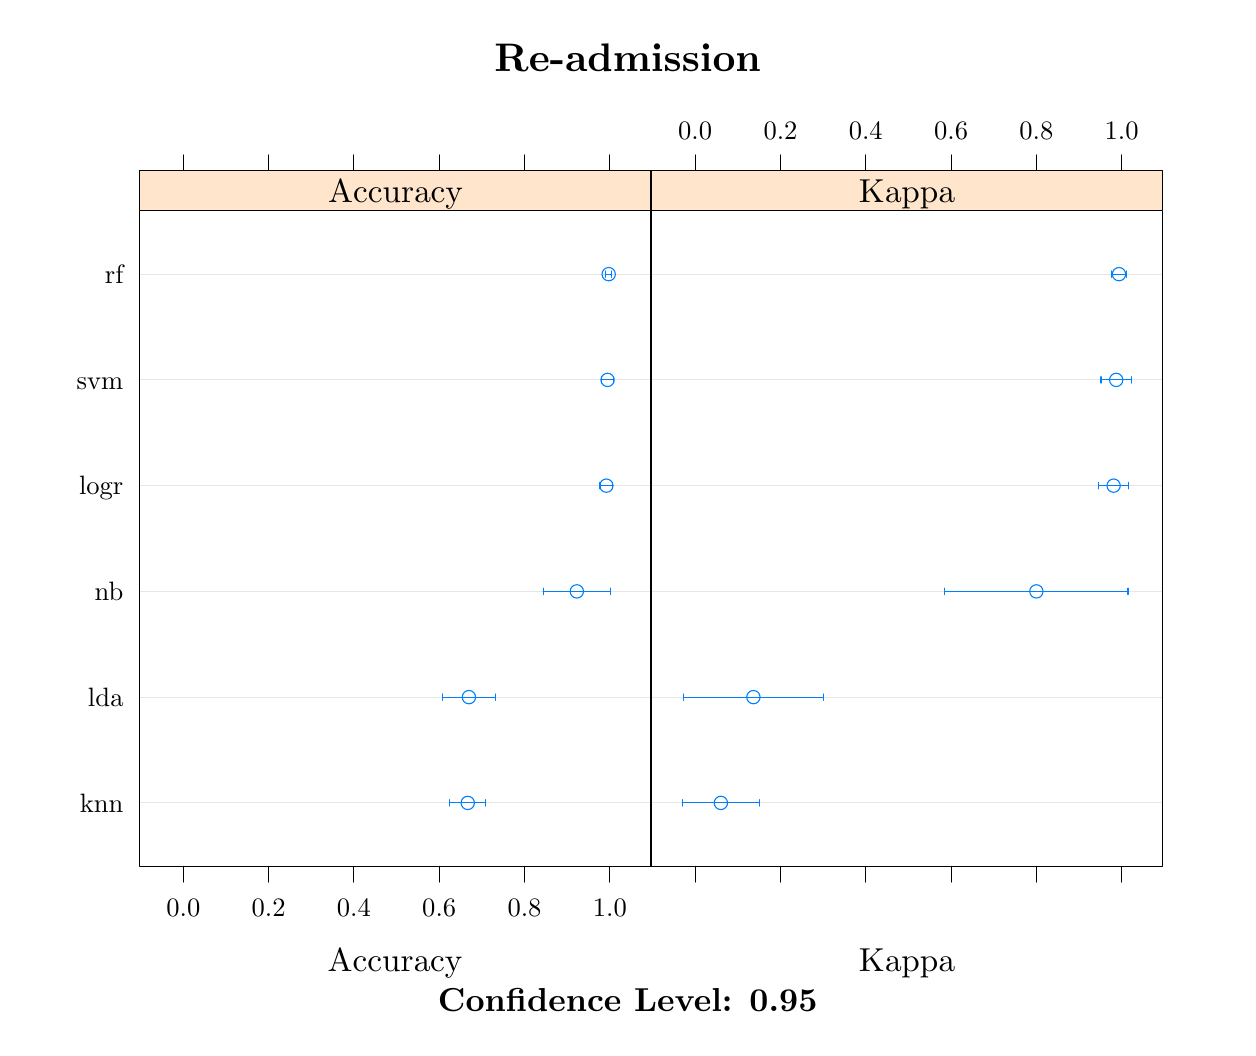
\begin{tikzpicture}[x=1pt,y=1pt]
\definecolor{fillColor}{RGB}{255,255,255}
\path[use as bounding box,fill=fillColor,fill opacity=0.00] (0,0) rectangle (433.62,361.35);
\begin{scope}
\path[clip] (  0.00,  0.00) rectangle (433.62,361.35);

\path[] (  0.00,  0.00) rectangle (433.62,361.35);
\definecolor{drawColor}{RGB}{0,0,0}

\node[text=drawColor,anchor=base,inner sep=0pt, outer sep=0pt, scale=  1.44] at (216.81,345.39) {\bfseries Re-admission};
\end{scope}
\begin{scope}
\path[clip] (  0.00,  0.00) rectangle (433.62,361.35);
\definecolor{drawColor}{RGB}{0,0,0}

\node[text=drawColor,anchor=base,inner sep=0pt, outer sep=0pt, scale=  1.20] at (216.81,  6.02) {\bfseries Confidence Level: 0.95};
\end{scope}
\begin{scope}
\path[clip] (  0.00,  0.00) rectangle (433.62,361.35);
\definecolor{drawColor}{RGB}{0,0,0}

\node[text=drawColor,anchor=base,inner sep=0pt, outer sep=0pt, scale=  1.20] at (132.76, 20.33) {Accuracy};

\node[text=drawColor,anchor=base,inner sep=0pt, outer sep=0pt, scale=  1.20] at (317.71, 20.33) {Kappa};
\end{scope}
\begin{scope}
\path[clip] (  0.00,  0.00) rectangle (433.62,361.35);
\definecolor{drawColor}{RGB}{0,0,0}

\path[draw=drawColor,line width= 0.4pt,line join=round,line cap=round] ( 56.24,309.66) -- ( 56.24,315.35);

\path[draw=drawColor,line width= 0.4pt,line join=round,line cap=round] ( 87.07,309.66) -- ( 87.07,315.35);

\path[draw=drawColor,line width= 0.4pt,line join=round,line cap=round] (117.89,309.66) -- (117.89,315.35);

\path[draw=drawColor,line width= 0.4pt,line join=round,line cap=round] (148.71,309.66) -- (148.71,315.35);

\path[draw=drawColor,line width= 0.4pt,line join=round,line cap=round] (179.54,309.66) -- (179.54,315.35);

\path[draw=drawColor,line width= 0.4pt,line join=round,line cap=round] (210.36,309.66) -- (210.36,315.35);
\end{scope}
\begin{scope}
\path[clip] (  0.00,  0.00) rectangle (433.62,361.35);
\definecolor{drawColor}{RGB}{0,0,0}

\node[text=drawColor,anchor=base east,inner sep=0pt, outer sep=0pt, scale=  0.96] at ( 34.58, 77.92) {knn};

\node[text=drawColor,anchor=base east,inner sep=0pt, outer sep=0pt, scale=  0.96] at ( 34.58,116.13) {lda};

\node[text=drawColor,anchor=base east,inner sep=0pt, outer sep=0pt, scale=  0.96] at ( 34.58,154.34) {nb};

\node[text=drawColor,anchor=base east,inner sep=0pt, outer sep=0pt, scale=  0.96] at ( 34.58,192.55) {logr};

\node[text=drawColor,anchor=base east,inner sep=0pt, outer sep=0pt, scale=  0.96] at ( 34.58,230.76) {svm};

\node[text=drawColor,anchor=base east,inner sep=0pt, outer sep=0pt, scale=  0.96] at ( 34.58,268.97) {rf};
\end{scope}
\begin{scope}
\path[clip] (  0.00,  0.00) rectangle (433.62,361.35);
\definecolor{drawColor}{RGB}{0,0,0}

\path[draw=drawColor,line width= 0.4pt,line join=round,line cap=round] ( 56.24, 58.30) -- ( 56.24, 52.61);

\path[draw=drawColor,line width= 0.4pt,line join=round,line cap=round] ( 87.07, 58.30) -- ( 87.07, 52.61);

\path[draw=drawColor,line width= 0.4pt,line join=round,line cap=round] (117.89, 58.30) -- (117.89, 52.61);

\path[draw=drawColor,line width= 0.4pt,line join=round,line cap=round] (148.71, 58.30) -- (148.71, 52.61);

\path[draw=drawColor,line width= 0.4pt,line join=round,line cap=round] (179.54, 58.30) -- (179.54, 52.61);

\path[draw=drawColor,line width= 0.4pt,line join=round,line cap=round] (210.36, 58.30) -- (210.36, 52.61);

\node[text=drawColor,anchor=base,inner sep=0pt, outer sep=0pt, scale=  0.96] at ( 56.24, 40.30) {0.0};

\node[text=drawColor,anchor=base,inner sep=0pt, outer sep=0pt, scale=  0.96] at ( 87.07, 40.30) {0.2};

\node[text=drawColor,anchor=base,inner sep=0pt, outer sep=0pt, scale=  0.96] at (117.89, 40.30) {0.4};

\node[text=drawColor,anchor=base,inner sep=0pt, outer sep=0pt, scale=  0.96] at (148.71, 40.30) {0.6};

\node[text=drawColor,anchor=base,inner sep=0pt, outer sep=0pt, scale=  0.96] at (179.54, 40.30) {0.8};

\node[text=drawColor,anchor=base,inner sep=0pt, outer sep=0pt, scale=  0.96] at (210.36, 40.30) {1.0};
\end{scope}
\begin{scope}
\path[clip] ( 40.28, 58.30) rectangle (225.23,295.21);
\definecolor{drawColor}{RGB}{230,230,230}

\path[draw=drawColor,line width= 0.4pt,line join=round,line cap=round] ( 40.28, 81.22) -- (225.23, 81.22);

\path[draw=drawColor,line width= 0.4pt,line join=round,line cap=round] ( 40.28,119.44) -- (225.23,119.44);

\path[draw=drawColor,line width= 0.4pt,line join=round,line cap=round] ( 40.28,157.65) -- (225.23,157.65);

\path[draw=drawColor,line width= 0.4pt,line join=round,line cap=round] ( 40.28,195.86) -- (225.23,195.86);

\path[draw=drawColor,line width= 0.4pt,line join=round,line cap=round] ( 40.28,234.07) -- (225.23,234.07);

\path[draw=drawColor,line width= 0.4pt,line join=round,line cap=round] ( 40.28,272.28) -- (225.23,272.28);
\definecolor{drawColor}{RGB}{0,128,255}

\path[draw=drawColor,line width= 0.4pt,line join=round,line cap=round] (159.02, 81.22) circle (  2.41);

\path[draw=drawColor,line width= 0.4pt,line join=round,line cap=round] (159.45,119.44) circle (  2.41);

\path[draw=drawColor,line width= 0.4pt,line join=round,line cap=round] (198.43,157.65) circle (  2.41);

\path[draw=drawColor,line width= 0.4pt,line join=round,line cap=round] (209.11,195.86) circle (  2.41);

\path[draw=drawColor,line width= 0.4pt,line join=round,line cap=round] (209.54,234.07) circle (  2.41);

\path[draw=drawColor,line width= 0.4pt,line join=round,line cap=round] (209.95,272.28) circle (  2.41);

\path[draw=drawColor,line width= 0.4pt,line join=round,line cap=round] (152.52, 81.22) -- (165.51, 81.22);

\path[draw=drawColor,line width= 0.4pt,line join=round,line cap=round] (150.00,119.44) -- (168.90,119.44);

\path[draw=drawColor,line width= 0.4pt,line join=round,line cap=round] (186.28,157.65) -- (210.59,157.65);

\path[draw=drawColor,line width= 0.4pt,line join=round,line cap=round] (206.81,195.86) -- (211.42,195.86);

\path[draw=drawColor,line width= 0.4pt,line join=round,line cap=round] (207.25,234.07) -- (211.82,234.07);

\path[draw=drawColor,line width= 0.4pt,line join=round,line cap=round] (208.81,272.28) -- (211.09,272.28);

\path[draw=drawColor,line width= 0.4pt,line join=round,line cap=round] (152.52, 82.37) -- (152.52, 80.08);

\path[draw=drawColor,line width= 0.4pt,line join=round,line cap=round] (150.00,120.58) -- (150.00,118.29);

\path[draw=drawColor,line width= 0.4pt,line join=round,line cap=round] (186.28,158.79) -- (186.28,156.50);

\path[draw=drawColor,line width= 0.4pt,line join=round,line cap=round] (206.81,197.00) -- (206.81,194.71);

\path[draw=drawColor,line width= 0.4pt,line join=round,line cap=round] (207.25,235.22) -- (207.25,232.92);

\path[draw=drawColor,line width= 0.4pt,line join=round,line cap=round] (208.81,273.43) -- (208.81,271.13);

\path[draw=drawColor,line width= 0.4pt,line join=round,line cap=round] (165.51, 82.37) -- (165.51, 80.08);

\path[draw=drawColor,line width= 0.4pt,line join=round,line cap=round] (168.90,120.58) -- (168.90,118.29);

\path[draw=drawColor,line width= 0.4pt,line join=round,line cap=round] (210.59,158.79) -- (210.59,156.50);

\path[draw=drawColor,line width= 0.4pt,line join=round,line cap=round] (211.42,197.00) -- (211.42,194.71);

\path[draw=drawColor,line width= 0.4pt,line join=round,line cap=round] (211.82,235.22) -- (211.82,232.92);

\path[draw=drawColor,line width= 0.4pt,line join=round,line cap=round] (211.09,273.43) -- (211.09,271.13);
\end{scope}
\begin{scope}
\path[clip] (  0.00,  0.00) rectangle (433.62,361.35);
\definecolor{drawColor}{RGB}{0,0,0}

\path[draw=drawColor,line width= 0.4pt,line join=round,line cap=round] ( 40.28, 58.30) rectangle (225.23,295.21);
\end{scope}
\begin{scope}
\path[clip] ( 40.28,295.21) rectangle (225.23,309.66);
\definecolor{drawColor}{RGB}{255,229,204}
\definecolor{fillColor}{RGB}{255,229,204}

\path[draw=drawColor,line width= 0.4pt,line join=round,line cap=round,fill=fillColor] ( 40.28,295.21) rectangle (225.23,309.66);
\definecolor{drawColor}{RGB}{0,0,0}

\node[text=drawColor,anchor=base west,inner sep=0pt, outer sep=0pt, scale=  1.20] at (108.58,298.30) {Accuracy};
\end{scope}
\begin{scope}
\path[clip] (  0.00,  0.00) rectangle (433.62,361.35);
\definecolor{drawColor}{RGB}{0,0,0}

\path[draw=drawColor,line width= 0.4pt,line join=round,line cap=round] ( 40.28,295.21) rectangle (225.23,309.66);
\end{scope}
\begin{scope}
\path[clip] (  0.00,  0.00) rectangle (433.62,361.35);
\definecolor{drawColor}{RGB}{0,0,0}

\path[draw=drawColor,line width= 0.4pt,line join=round,line cap=round] (241.20,309.66) -- (241.20,315.35);

\path[draw=drawColor,line width= 0.4pt,line join=round,line cap=round] (272.03,309.66) -- (272.03,315.35);

\path[draw=drawColor,line width= 0.4pt,line join=round,line cap=round] (302.85,309.66) -- (302.85,315.35);

\path[draw=drawColor,line width= 0.4pt,line join=round,line cap=round] (333.67,309.66) -- (333.67,315.35);

\path[draw=drawColor,line width= 0.4pt,line join=round,line cap=round] (364.50,309.66) -- (364.50,315.35);

\path[draw=drawColor,line width= 0.4pt,line join=round,line cap=round] (395.32,309.66) -- (395.32,315.35);

\node[text=drawColor,anchor=base,inner sep=0pt, outer sep=0pt, scale=  0.96] at (241.20,321.04) {0.0};

\node[text=drawColor,anchor=base,inner sep=0pt, outer sep=0pt, scale=  0.96] at (272.03,321.04) {0.2};

\node[text=drawColor,anchor=base,inner sep=0pt, outer sep=0pt, scale=  0.96] at (302.85,321.04) {0.4};

\node[text=drawColor,anchor=base,inner sep=0pt, outer sep=0pt, scale=  0.96] at (333.67,321.04) {0.6};

\node[text=drawColor,anchor=base,inner sep=0pt, outer sep=0pt, scale=  0.96] at (364.50,321.04) {0.8};

\node[text=drawColor,anchor=base,inner sep=0pt, outer sep=0pt, scale=  0.96] at (395.32,321.04) {1.0};
\end{scope}
\begin{scope}
\path[clip] (  0.00,  0.00) rectangle (433.62,361.35);
\definecolor{drawColor}{RGB}{0,0,0}

\path[draw=drawColor,line width= 0.4pt,line join=round,line cap=round] (241.20, 58.30) -- (241.20, 52.61);

\path[draw=drawColor,line width= 0.4pt,line join=round,line cap=round] (272.03, 58.30) -- (272.03, 52.61);

\path[draw=drawColor,line width= 0.4pt,line join=round,line cap=round] (302.85, 58.30) -- (302.85, 52.61);

\path[draw=drawColor,line width= 0.4pt,line join=round,line cap=round] (333.67, 58.30) -- (333.67, 52.61);

\path[draw=drawColor,line width= 0.4pt,line join=round,line cap=round] (364.50, 58.30) -- (364.50, 52.61);

\path[draw=drawColor,line width= 0.4pt,line join=round,line cap=round] (395.32, 58.30) -- (395.32, 52.61);
\end{scope}
\begin{scope}
\path[clip] (225.23, 58.30) rectangle (410.19,295.21);
\definecolor{drawColor}{RGB}{230,230,230}

\path[draw=drawColor,line width= 0.4pt,line join=round,line cap=round] (225.23, 81.22) -- (410.19, 81.22);

\path[draw=drawColor,line width= 0.4pt,line join=round,line cap=round] (225.23,119.44) -- (410.19,119.44);

\path[draw=drawColor,line width= 0.4pt,line join=round,line cap=round] (225.23,157.65) -- (410.19,157.65);

\path[draw=drawColor,line width= 0.4pt,line join=round,line cap=round] (225.23,195.86) -- (410.19,195.86);

\path[draw=drawColor,line width= 0.4pt,line join=round,line cap=round] (225.23,234.07) -- (410.19,234.07);

\path[draw=drawColor,line width= 0.4pt,line join=round,line cap=round] (225.23,272.28) -- (410.19,272.28);
\definecolor{drawColor}{RGB}{0,128,255}

\path[draw=drawColor,line width= 0.4pt,line join=round,line cap=round] (250.49, 81.22) circle (  2.41);

\path[draw=drawColor,line width= 0.4pt,line join=round,line cap=round] (262.24,119.44) circle (  2.41);

\path[draw=drawColor,line width= 0.4pt,line join=round,line cap=round] (364.49,157.65) circle (  2.41);

\path[draw=drawColor,line width= 0.4pt,line join=round,line cap=round] (392.40,195.86) circle (  2.41);

\path[draw=drawColor,line width= 0.4pt,line join=round,line cap=round] (393.34,234.07) circle (  2.41);

\path[draw=drawColor,line width= 0.4pt,line join=round,line cap=round] (394.34,272.28) circle (  2.41);

\path[draw=drawColor,line width= 0.4pt,line join=round,line cap=round] (236.59, 81.22) -- (264.38, 81.22);

\path[draw=drawColor,line width= 0.4pt,line join=round,line cap=round] (237.02,119.44) -- (287.45,119.44);

\path[draw=drawColor,line width= 0.4pt,line join=round,line cap=round] (331.38,157.65) -- (397.60,157.65);

\path[draw=drawColor,line width= 0.4pt,line join=round,line cap=round] (387.00,195.86) -- (397.80,195.86);

\path[draw=drawColor,line width= 0.4pt,line join=round,line cap=round] (387.84,234.07) -- (398.84,234.07);

\path[draw=drawColor,line width= 0.4pt,line join=round,line cap=round] (391.62,272.28) -- (397.06,272.28);

\path[draw=drawColor,line width= 0.4pt,line join=round,line cap=round] (236.59, 82.37) -- (236.59, 80.08);

\path[draw=drawColor,line width= 0.4pt,line join=round,line cap=round] (237.02,120.58) -- (237.02,118.29);

\path[draw=drawColor,line width= 0.4pt,line join=round,line cap=round] (331.38,158.79) -- (331.38,156.50);

\path[draw=drawColor,line width= 0.4pt,line join=round,line cap=round] (387.00,197.00) -- (387.00,194.71);

\path[draw=drawColor,line width= 0.4pt,line join=round,line cap=round] (387.84,235.22) -- (387.84,232.92);

\path[draw=drawColor,line width= 0.4pt,line join=round,line cap=round] (391.62,273.43) -- (391.62,271.13);

\path[draw=drawColor,line width= 0.4pt,line join=round,line cap=round] (264.38, 82.37) -- (264.38, 80.08);

\path[draw=drawColor,line width= 0.4pt,line join=round,line cap=round] (287.45,120.58) -- (287.45,118.29);

\path[draw=drawColor,line width= 0.4pt,line join=round,line cap=round] (397.60,158.79) -- (397.60,156.50);

\path[draw=drawColor,line width= 0.4pt,line join=round,line cap=round] (397.80,197.00) -- (397.80,194.71);

\path[draw=drawColor,line width= 0.4pt,line join=round,line cap=round] (398.84,235.22) -- (398.84,232.92);

\path[draw=drawColor,line width= 0.4pt,line join=round,line cap=round] (397.06,273.43) -- (397.06,271.13);
\end{scope}
\begin{scope}
\path[clip] (  0.00,  0.00) rectangle (433.62,361.35);
\definecolor{drawColor}{RGB}{0,0,0}

\path[draw=drawColor,line width= 0.4pt,line join=round,line cap=round] (225.23, 58.30) rectangle (410.19,295.21);
\end{scope}
\begin{scope}
\path[clip] (225.23,295.21) rectangle (410.19,309.66);
\definecolor{drawColor}{RGB}{255,229,204}
\definecolor{fillColor}{RGB}{255,229,204}

\path[draw=drawColor,line width= 0.4pt,line join=round,line cap=round,fill=fillColor] (225.23,295.21) rectangle (410.19,309.66);
\definecolor{drawColor}{RGB}{0,0,0}

\node[text=drawColor,anchor=base west,inner sep=0pt, outer sep=0pt, scale=  1.20] at (300.39,298.30) {Kappa};
\end{scope}
\begin{scope}
\path[clip] (  0.00,  0.00) rectangle (433.62,361.35);
\definecolor{drawColor}{RGB}{0,0,0}

\path[draw=drawColor,line width= 0.4pt,line join=round,line cap=round] (225.23,295.21) rectangle (410.19,309.66);
\end{scope}
\end{tikzpicture}
}
    \caption[Bi-classification of re-admission as clinical outcome]{\textit{Bi-classification of re-admission as clinical outcome}}
    \label{fig:bi_class_read}
\end{figure}

\noindent are illustrated in Figure (\ref{fig:bi_class_read}) and Table (\ref{tab:class_readmission}). The results are very much different than what we found with the mortality classification. Surprisingly, three algorithms seem to distinguish themselves from the others, namely the random forest (\texttt{rf}), support vector machines (\texttt{svm}) and logistic regression (\texttt{logr}). Interestingly, all three of these algorithm score very high both in terms of accuracy and kappa. The algorithm with the most promising results is the random forest. It has an estimated mean prediction accuracy of 99.7\% with a kappa of 0.994. The random forest is found to be the most superior classification algorithm in both predicting mortality and re-admission. This is not uncommon as in the literature there are many studies that report of the random forest as being a very effective algorithm for classifying clinical outcomes, see e.g. \cite{austin2013using} and \cite{zolfaghar2013big}. The next algorithm that show potential in predicting re-admission is the support vector machines (\texttt{svm}) algorithm. It has an estimated mean accuracy of 99.5\% with a kappa of 0.987. We consider this to be interesting as in the previous section we found that the SVM was one of the lowest performing algorithms when it comes to predicting mortality. The last algorithm that show potential is that of the logistic regression (\texttt{logr}). The estimated mean accuracy for this algorithm was 99.2\% with a kappa of 0.981. In addition to having a very good accuracy and kappa, its worth mentioning that given is level of simplicity, one can argue that the  

\vspace*{-0,1cm}\begin{footnotesize}
\begin{tabularx}{\textwidth}{LLLLLLLL}
\caption{Summary statistics re-admission classification}\label{tab:class_readmission}\\
\toprule
 & Min. & 1st Qu. & Median & Mean & 3rd Qu. & Max. & NA's \\ 
\midrule
\endfirsthead
\caption*{\textbf{Table \ref{tab:class_readmission}:} Summary statistics re-admission classification (\textit{continued})}\\
\toprule
 & Min. & 1st Qu. & Median & Mean & 3rd Qu. & Max. & NA's \\ 
\midrule
\endhead
\multicolumn{8}{c}{PANEL I: Accuracy}\\
\midrule
knn & 0.595 & 0.609 & 0.654 & 0.658 & 0.698 & 0.737 & 0.000 \\ 
lda & 0.568 & 0.649 & 0.694 & 0.688 & 0.735 & 0.763 & 0.000 \\ 
nb & 0.838 & 0.921 & 0.960 & 0.947 & 0.974 & 1.000 & 0.000 \\ 
logr & 0.946 & 0.980 & 1.000 & 0.989 & 1.000 & 1.000 & 0.000 \\ 
svm & 0.973 & 1.000 & 1.000 & 0.997 & 1.000 & 1.000 & 0.000 \\ 
rf & 0.973 & 1.000 & 1.000 & 0.997 & 1.000 & 1.000 & 0.000 \\ 
\midrule
\multicolumn{8}{c}{PANEL II: Kappa}\\
\midrule
knn & -0.183 & -0.106 & 0.020 & 0.028 & 0.124 & 0.258 & 0.000 \\ 
lda & -0.101 & 0.037 & 0.193 & 0.168 & 0.327 & 0.408 & 0.000 \\ 
nb & 0.539 & 0.806 & 0.899 & 0.863 & 0.937 & 1.000 & 0.000 \\ 
logr & 0.877 & 0.955 & 1.000 & 0.975 & 1.000 & 1.000 & 0.000 \\ 
svm & 0.934 & 1.000 & 1.000 & 0.993 & 1.000 & 1.000 & 0.000 \\ 
rf & 0.934 & 1.000 & 1.000 & 0.993 & 1.000 & 1.000 & 0.000 \\
\midrule
\end{tabularx}
\end{footnotesize}

\noindent logistic regression algorithm is more preferable to more advanced classification algorithm. In both the cases that we have examined, we have found that the random forest and the logistic regression algorithm perform decently. Both algorithms are also very different in terms of their level of complexity. They are also very much used in the literature and is often a favourite among practitioners of medical statistical analysis, see e.g. \cite{austin2013using}, \cite{zolfaghar2013big}, \cite{shah2014phenomapping} and \cite{panahiazar2015using}. Accordingly, we have reasons to believe that both the random forest and the logistic regression are the two main algorithms that show the most potential in predicting both the mortality and re-admission of HF patients.

\section{Discussion}

\noindent The objective of this was two fold: (i) we attempted to give a though analysis of how well various clustering algorithms (Hierarchical, K-Means and Expectation-Maximization) perform in producing phenotypically distinct clinical patient groups (i.e. phenomapping) with HFpEF and HFmrEF. Our strategy for answering this research question has been to compare the level of dissimilarity between patient groups that are produced at two levels. Firstly, we looked at the Bi-clustering problem where we compared the patient groups produced by the algorithms with that of the physicians. We found that if one assumes that the clustering algorithm that produces the most significantly different baseline characteristics as being the optimal. Then we have reasons to believe that the Hierarchical and K-Means clustering algorithms show signs of being a tool that physicians can use to cross-check their assumptions and diagnosis in order to further improve the diagnosis of patients with the preserved and mid-range subtypes of HF. Overall these algorithms produce 62 significantly different baseline characteristics compared to 59 produced by the physians. Secondly, we looked at how well the clustering algorithms performed in producing "new" patient groups within both subtypes of HF. We analyzed this by attempting to re-cluster patient groups from both the subtypes produced by the physicians and the ML algorithms. 

\end{document}